\begin{figure}
  \centering
  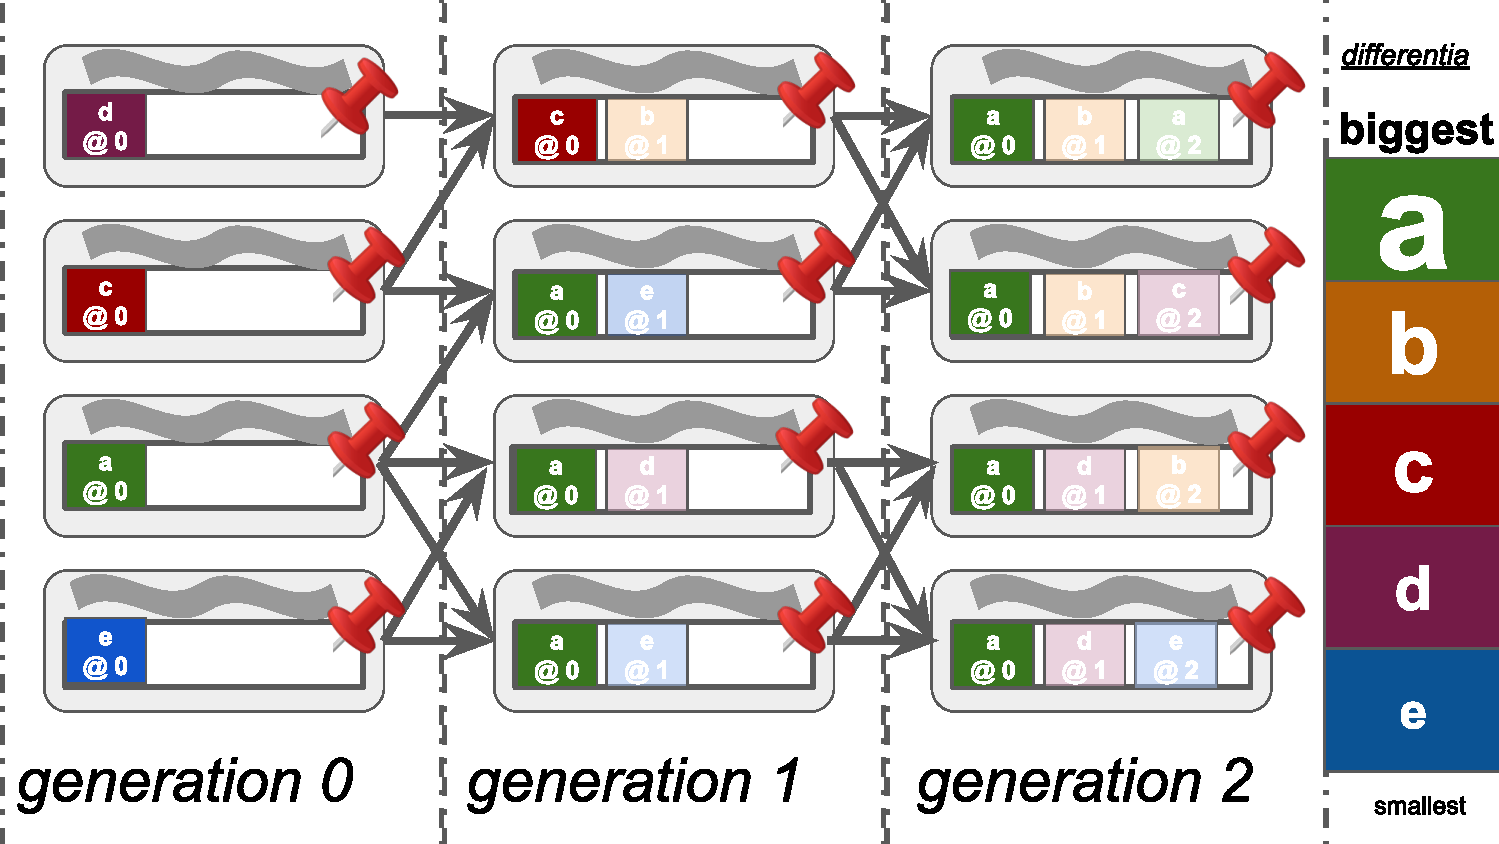
\includegraphics[width=\textwidth]{img/gene-drive}
  \caption{
    Gene drive mechanism to enforce hereditary stratigraph instrumentation consistency within a species (i.e., an interbreeding population).
    When two parents recombine, the larger of the parents' differentia values at each layer is inherited.
    The largest value generated among layer 0 differentia ($a$) happens to occur in only one member of generation 0.
    Through the gene drive mechanism, this differentia value is inherited by all offspring of the originating organism.
    By generation 2, the differentia value has swept layer 0 and will remain fixed permanently.
    This mechanism applies to ``species-level'' instrumentation (Figure \ref{fig:annotation-types}).
  }
  \label{fig:gene-drive}
\end{figure}
